\documentclass[tikz,border=6pt]{standalone}
\usepackage[T1]{fontenc}
\usepackage[utf8]{inputenc}
\usepackage{pgfplots}
\pgfplotsset{compat=1.18}
\begin{document}
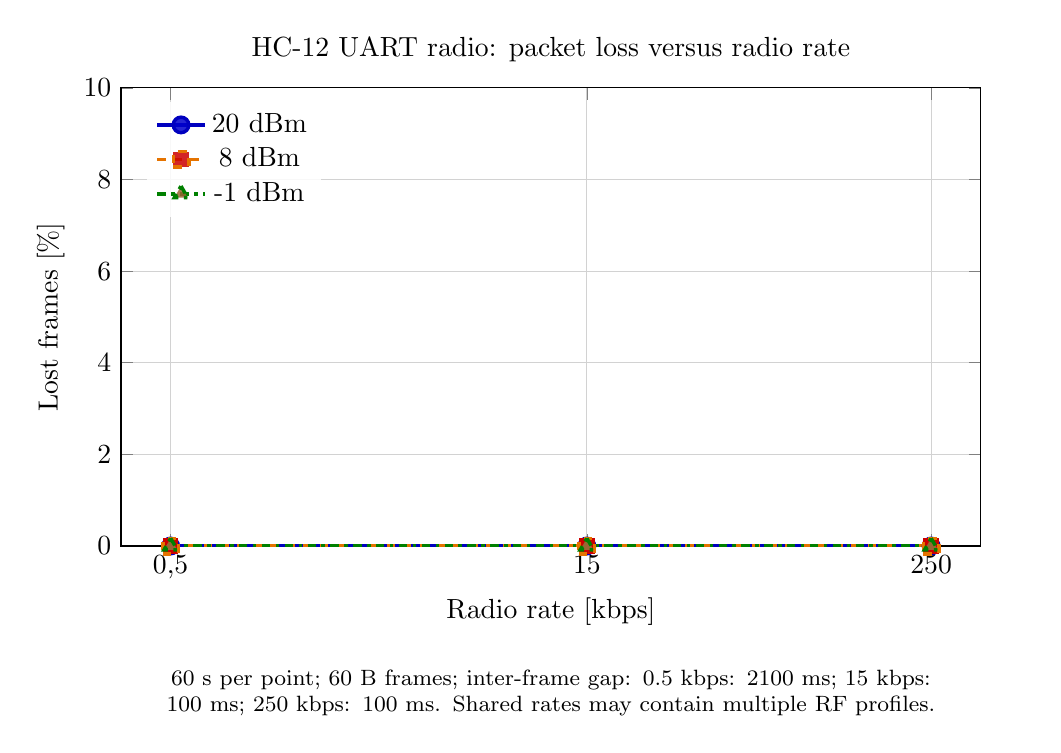
\begin{tikzpicture}
\begin{axis}[width=12.5cm, height=7.4cm,
  title={HC-12 UART radio: packet loss versus radio rate},
  xmode=log, log basis x=10,
  xmin=0.333333333, xmax=375, xtick={0.5,15,250},
  xticklabels={0{,}5,15,250}, ymin=0, ymax=10,
  xlabel={Radio rate [kbps]}, ylabel={Lost frames [\%]},
  grid=both, minor grid style={gray!15}, major grid style={gray!35},
  every axis plot/.append style={line width=1.25pt, mark size=2.8pt},
  legend style={draw=none, fill=white, fill opacity=0.85, text opacity=1,
    at={(0.03,0.97)}, anchor=north west, legend columns=1},
]
\addplot+[blue!75!black, solid, mark=*] coordinates {(0.5,0) (15,0) (250,0)};
\addlegendentry{20 dBm}
\addplot+[orange!90!black, dashed, mark=square*] coordinates {(0.5,0) (15,0) (250,0)};
\addlegendentry{8 dBm}
\addplot+[green!50!black, dashdotted, mark=triangle*] coordinates {(0.5,0) (15,0) (250,0)};
\addlegendentry{-1 dBm}
\end{axis}
\node[font=\footnotesize, align=center, text width=12cm, anchor=north]
  at ([yshift=-1.45cm]current axis.south)
  {60 s per point; 60 B frames; inter-frame gap: 0.5 kbps: 2100 ms; 15 kbps: 100 ms; 250 kbps: 100 ms. Shared rates may contain multiple RF profiles.};
\end{tikzpicture}
\end{document}
